\documentclass[aspectratio=169,11pt]{beamer}
\usepackage[utf8]{inputenc}
\usepackage[T1]{fontenc}
\usepackage[spanish]{babel}
\usepackage{amsmath,amssymb}
\usepackage{tikz}
\usetikzlibrary{arrows.meta,angles,calc,positioning}
\usetheme{Madrid}
\usecolortheme{default}
\setbeamertemplate{navigation symbols}{}
\setbeamertemplate{blocks}[rounded][shadow=false]
\newcommand{\ang}[1]{\angle #1^\circ}

\title[Nichols chart]{Paso 6: El Nichols chart}
\subtitle{$L(j\omega)$ en ejes (fase, dB), con el valor de $|T|$ escrito en el mapa}
\author{Curso de control robusto (QFT)}
\date{}
\begin{document}
\begin{frame}\titlepage\end{frame}

\begin{frame}{Dónde encaja este paso}
  \tiny
  \begin{enumerate}\setlength{\itemsep}{-2pt}
    \item[1.] Números complejos \hfill \textcolor{gray}{(hecho)}
    \item[2.] Funciones de transferencia: $s$, polos y ceros \hfill \textcolor{gray}{(hecho)}
    \item[3.] Respuesta en frecuencia: $s=j\omega$, magnitud y fase \hfill \textcolor{gray}{(hecho)}
    \item[4.] Decibelios y escala logarítmica (Bode) \hfill \textcolor{gray}{(hecho)}
    \item[5.] Realimentación: $L$, $T=\frac{L}{1+L}$, $S=\frac{1}{1+L}$ \hfill \textcolor{gray}{(hecho)}
    \item[\textbf{6.}] \textbf{Nichols chart} \hfill $\leftarrow$ estamos aquí
    \item[7.] Incertidumbre y templates
    \item[8.] Especificaciones $\rightarrow$ bounds
    \item[9.] Loop shaping, prefiltro y verificación
    \item[10.] QFT en control digital
    \item[11.] Dos caminos digitales: $z$ y $w$
    \item[12.] Estabilidad, límites, más especificaciones y caso real
    \item[13.] Muestreo por eventos con periodo base $T$
    \item[14.] Sistemas de dos estados: lazo interno y externo
    \item[15.] QFT y sistemas no lineales
    \item[16.] Algoritmos de QFT: cómo funcionan por dentro
    \item[17.] QFT en Python: una biblioteca paso a paso
    \item[18.] QFT en MATLAB: el mismo código, otra sintaxis
    \item[19.] Historia, panorama y bibliografía
  \end{enumerate}
  \vspace{4pt}
  \begin{block}{Objetivo de hoy}
    Entender qué es el Nichols chart: un mapa donde cada punto es un valor posible de $L(j\omega)$ y donde ya viene escrito cuánto vale $|T|=\left|\frac{L}{1+L}\right|$ en ese punto.
  \end{block}
\end{frame}

\begin{frame}{La idea: el mismo número complejo, otras coordenadas}
  \footnotesize
  \centering
  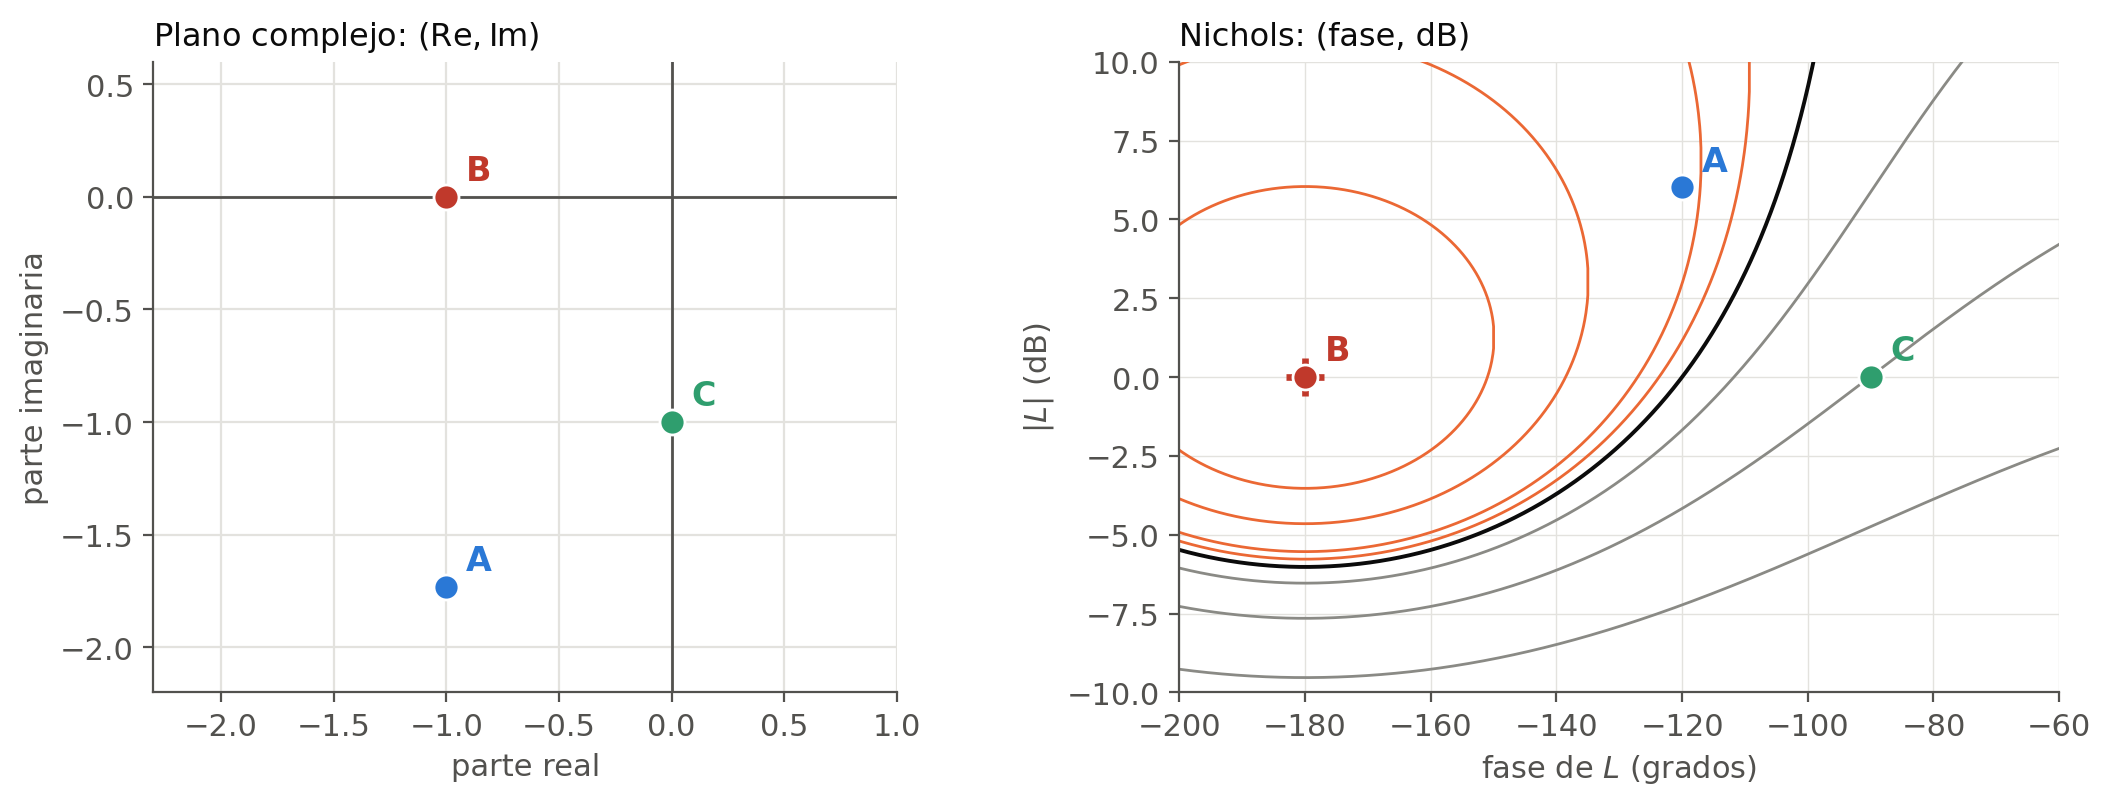
\includegraphics[width=0.86\textwidth]{fig/dos_planos.png}\\[2pt]
  \begin{tabular}{c|c|c|c}
    punto & complejo & polar & Nichols $(\angle L,\ |L|_{\text{dB}})$\\\hline
    {\color{blue}A} & $-1-1.732j$ & $2\angle-120^\circ$ & $(-120^\circ,\ 6.02\text{ dB})$\\
    {\color{red}B} & $-1$ & $1\angle-180^\circ$ & $(-180^\circ,\ 0\text{ dB})$\\
    {\color{green!50!black}C} & $-j$ & $1\angle-90^\circ$ & $(-90^\circ,\ 0\text{ dB})$
  \end{tabular}
\end{frame}

\begin{frame}{Por qué esos ejes: en Nichols, multiplicar es sumar}
  \small
  \begin{columns}[T]
  \begin{column}{0.52\textwidth}
    \begin{block}{Paso 4 en acción}
      $L=G\cdot P\ \Rightarrow\ |L|_{\text{dB}}=|G|_{\text{dB}}+|P|_{\text{dB}}$ y $\angle L=\angle G+\angle P$.
    \end{block}
    \textbf{Ejemplo en una frecuencia.}\\
    $P=0.5\angle-100^\circ$ \ $\to(-100^\circ,\ -6.02\text{ dB})$\\
    $G=4\angle-30^\circ$ \ $\to(-30^\circ,\ +12.04\text{ dB})$\\
    $L=GP=2\angle-130^\circ$ \ $\to(-130^\circ,\ +6.02\text{ dB})$\\[2pt]
    En el mapa: \textbf{sumar} un vector $(-30^\circ,+12\text{ dB})$ a la posición de $P$.
  \end{column}
  \begin{column}{0.46\textwidth}
    \begin{block}{Dos movimientos básicos}
      \begin{itemize}
        \item Subir/bajar la \textbf{ganancia}: mover el punto \emph{verticalmente}.
        \item Añadir \textbf{retardo} o un polo: mover el punto \emph{horizontalmente}, hacia la izquierda.
      \end{itemize}
    \end{block}
    \begin{alertblock}{Por qué es la herramienta de QFT}
      Diseñar $G$ es empujar $P$ por este mapa. En el plano complejo habría que multiplicar.
    \end{alertblock}
  \end{column}
  \end{columns}
\end{frame}

\begin{frame}{La pregunta: dado un punto del mapa, ¿cuánto vale $|T|$?}
  \small
  Sea $L=r\angle\theta$, es decir $L=r\cos\theta+j\,r\sin\theta$. Entonces
  \[ |1+L|^2=(1+r\cos\theta)^2+(r\sin\theta)^2=1+2r\cos\theta+r^2 \]
  \[ \boxed{\;|T|=\frac{|L|}{|1+L|}=\frac{r}{\sqrt{1+2r\cos\theta+r^2}}\;} \]
  \begin{block}{Qué significa}
    $|T|$ depende solo de $r=|L|$ y de $\theta=\angle L$, o sea, de la \textbf{posición del punto en el mapa de Nichols}. Podemos calcularlo en cada punto y escribir el resultado en el mapa.
  \end{block}
  \textcolor{gray}{Probemos con nueve puntos.}
\end{frame}

\begin{frame}{Rellenando el mapa: $|T|$ en dB en nueve puntos}
  \small
  \begin{columns}[T]
  \begin{column}{0.56\textwidth}
    \centering
    \begin{tabular}{c|c|c|c}
      $|L|$ \textbackslash\ $\angle L$ & $0^\circ$ & $-90^\circ$ & $-180^\circ$\\\hline
      $2$ ($+6.02$ dB) & $-3.52$ & $-0.97$ & $+6.02$\\
      $1$ ($0$ dB) & $-6.02$ & $-3.01$ & $\infty$\\
      $0.5$ ($-6.02$ dB) & $-9.54$ & $-6.99$ & $0$
    \end{tabular}
    \vspace{4pt}\\
    {\footnotesize (cada celda: $|T|$ en dB)}
  \end{column}
  \begin{column}{0.42\textwidth}
    \begin{itemize}
      \item $\theta=-180^\circ$, $r=1$: es el punto $-1$, $T\to\infty$.
      \item Lejos del punto crítico, $|T|<0$ dB y cae a medida que $L$ baja.
      \item Con muchos más puntos, los que tienen el \textbf{mismo} $|T|$ se unen en una curva.
    \end{itemize}
  \end{column}
  \end{columns}
  \begin{block}{Contorno de nivel}
    Una curva de $|T|=M$ constante, dibujada en (fase, dB). Es como las curvas de nivel de un mapa topográfico, pero con la altura $|T|$.
  \end{block}
\end{frame}

\begin{frame}{El Nichols chart}
  \footnotesize
  \begin{columns}[T]
  \begin{column}{0.66\textwidth}
    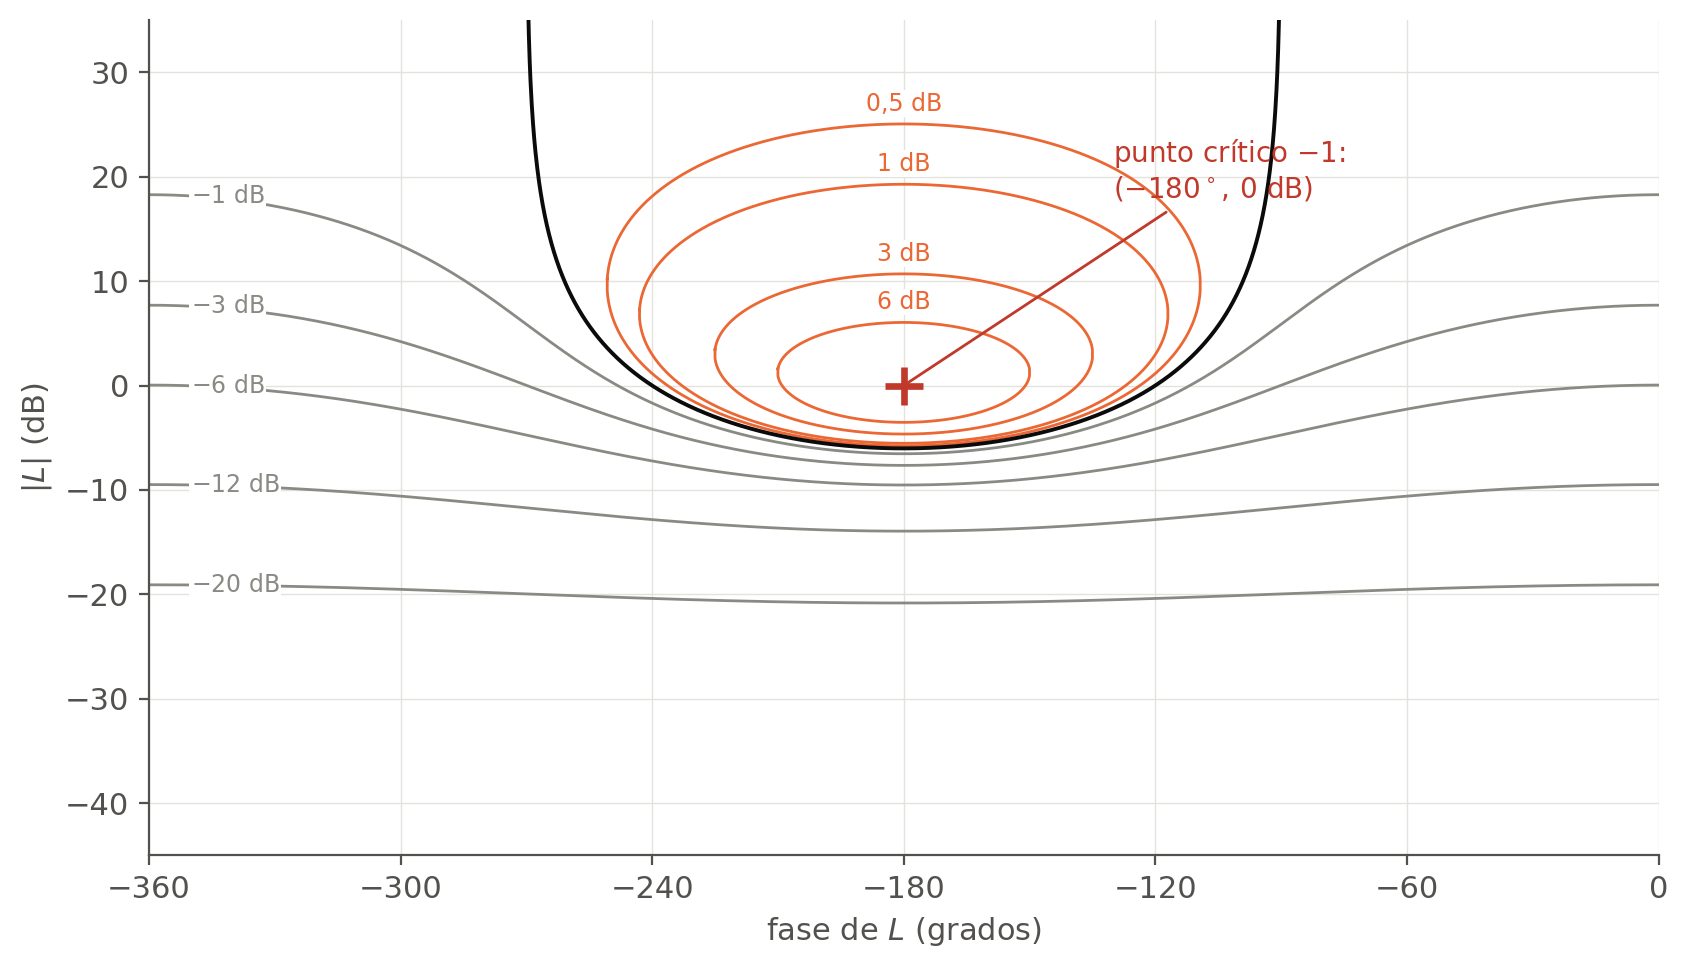
\includegraphics[width=\textwidth]{fig/carta.png}
  \end{column}
  \begin{column}{0.32\textwidth}
    \begin{block}{Qué se ve}
      \begin{itemize}
        \item \textbf{Óvalos naranja}: $|T|>0$ dB, alrededor del punto crítico. Más cerca, más alto.
        \item \textbf{Curva negra}: $|T|=0$ dB.
        \item \textbf{Curvas grises}: $|T|<0$ dB.
      \end{itemize}
    \end{block}
    \begin{alertblock}{El punto crítico}
      $+$ en $(-180^\circ,\ 0\text{ dB})$ es el punto $-1$ del paso 5.
    \end{alertblock}
    \textcolor{gray}{Cómo se dibujan (y los contornos de $\angle T$): apéndice.}
  \end{column}
  \end{columns}
\end{frame}

\begin{frame}{Cómo se lee cada zona}
  \small
  \begin{center}
  \begin{tabular}{p{0.25\textwidth}|p{0.6\textwidth}}
    \textbf{Zona} & \textbf{Qué le pasa a $T$}\\\hline
    Arriba ($|L|$ grande) & $|T|\approx0$ dB: $y$ sigue a $r$. Las curvas se aplastan contra la de 0 dB.\\[3pt]
    Alrededor de $(-180^\circ,0)$ & Óvalos de $|T|>0$ dB: \textbf{pico de resonancia}. Es la zona a evitar.\\[3pt]
    Abajo ($|L|$ pequeño) & $|T|\approx|L|$: las curvas son casi horizontales y $|T|_{\text{dB}}\approx|L|_{\text{dB}}$.
  \end{tabular}
  \end{center}
  \begin{block}{Regla de lectura}
    Para cada frecuencia, $L(j\omega)$ es un punto. Mira entre qué dos contornos cae: ese es $|T(j\omega)|$.
  \end{block}
\end{frame}

\begin{frame}{Un lazo real sobre la carta: $L(s)=\dfrac{3}{s\,(1+s/2)(1+s/10)}$}
  \footnotesize
  \begin{columns}[T]
  \begin{column}{0.62\textwidth}
    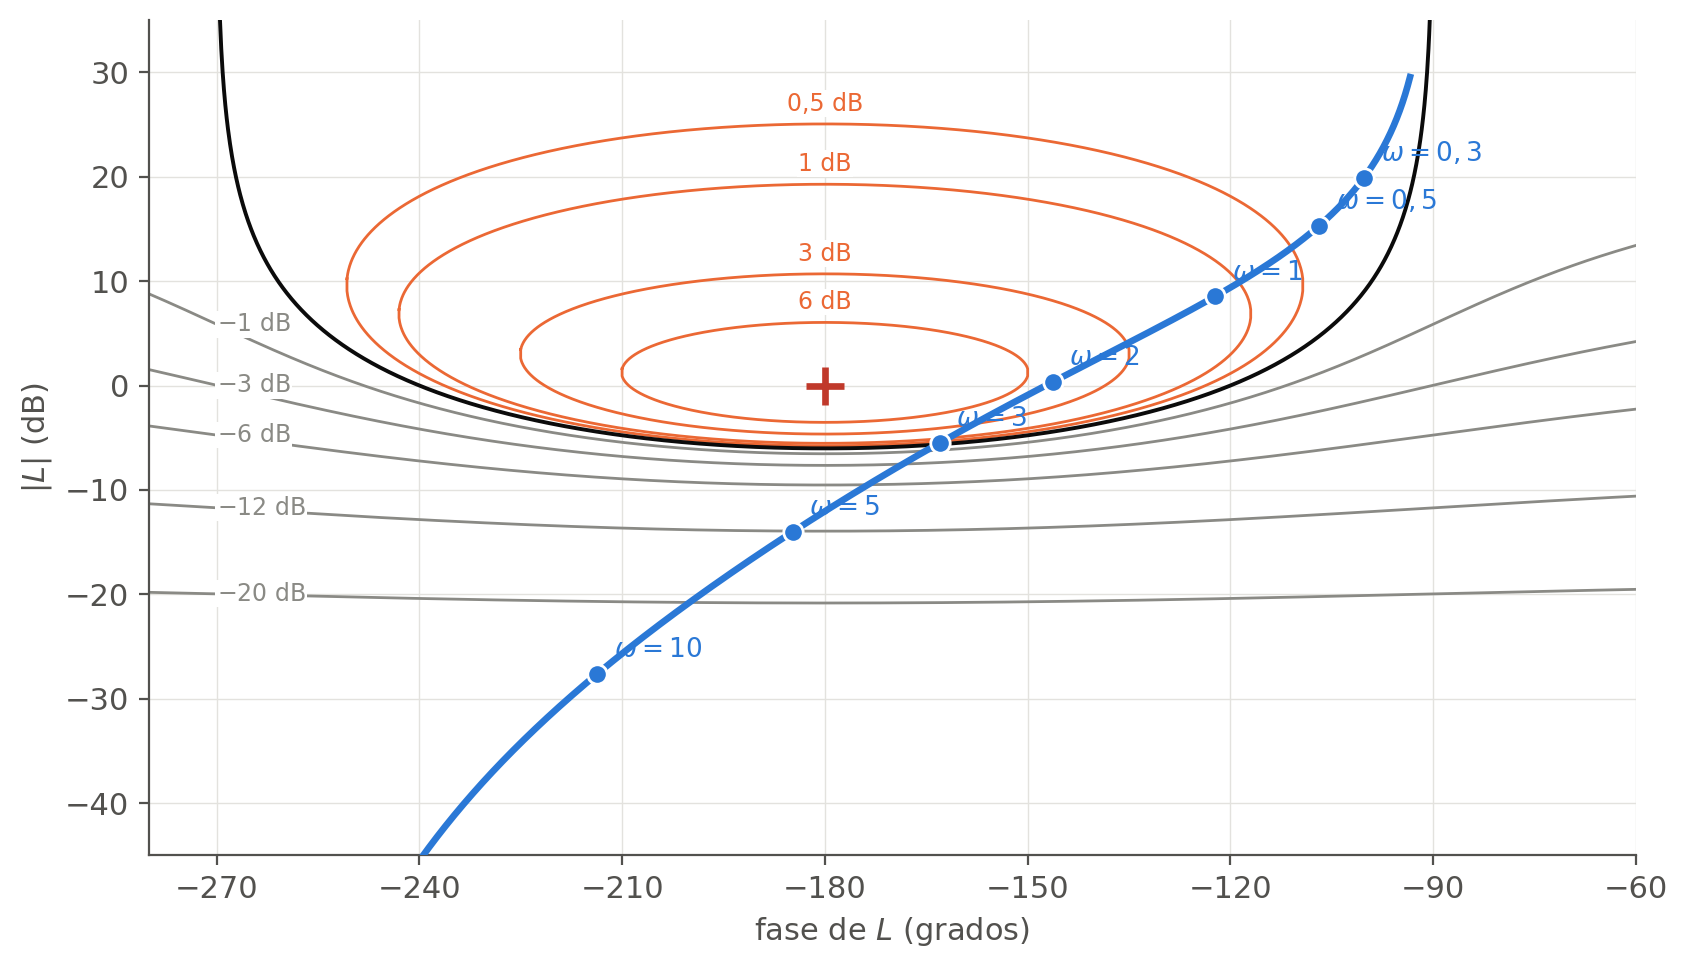
\includegraphics[width=\textwidth]{fig/nichols_L.png}
  \end{column}
  \begin{column}{0.36\textwidth}
    \centering
    \begin{tabular}{r|c|r}
      $\omega$ & lectura & calculado\\\hline
      1 & 1 a 3 dB & $1.3$\\
      2 & 3 a 6 dB & $4.9$\\
      3 & 0 a 0.5 dB & $0.26$\\
      5 & $\approx-12$ dB & $-12.1$
    \end{tabular}
    \vspace{3pt}
    \begin{block}{El pico de $T$}
      Es el contorno más alto que la curva \emph{toca}: aquí el de $5.1$ dB, cerca de $\omega=2$.
    \end{block}
  \end{column}
  \end{columns}
\end{frame}

\begin{frame}{Márgenes de estabilidad en Nichols}
  \footnotesize
  \begin{columns}[T]
  \begin{column}{0.62\textwidth}
    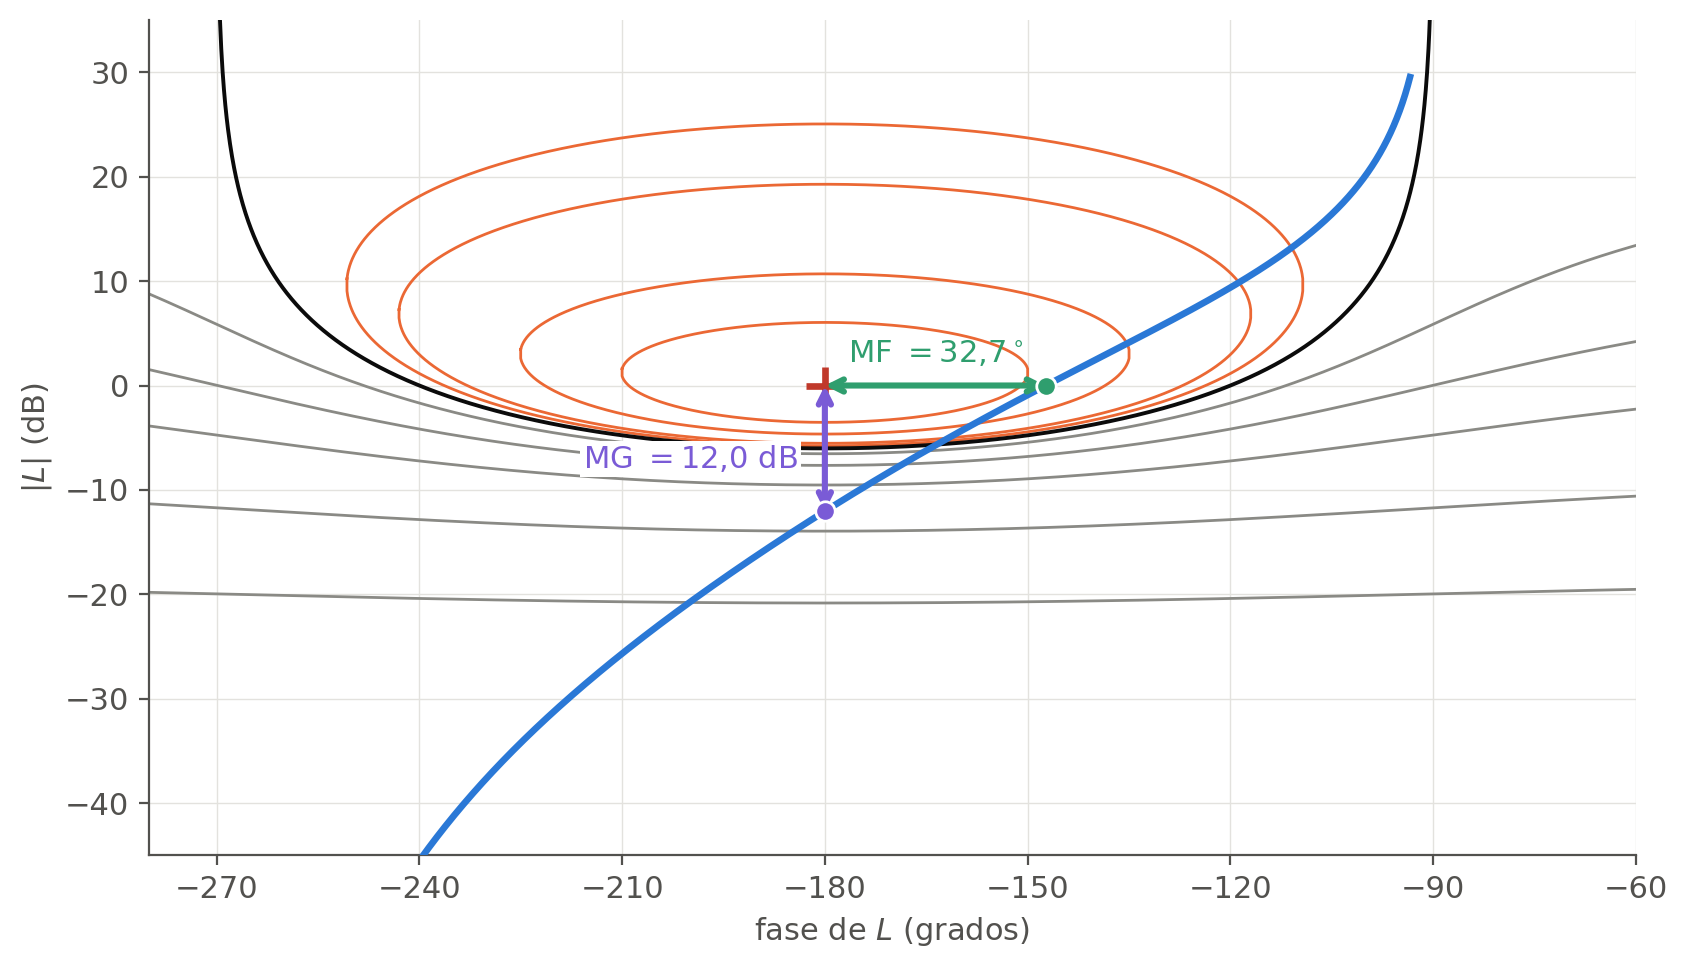
\includegraphics[width=\textwidth]{fig/margenes.png}
  \end{column}
  \begin{column}{0.36\textwidth}
    \begin{block}{Margen de fase}
      Distancia \textbf{horizontal} desde donde la curva cruza 0 dB hasta $-180^\circ$: aquí $32.7^\circ$ ($\omega_c=2.05$).
    \end{block}
    \begin{block}{Margen de ganancia}
      Distancia \textbf{vertical} desde donde la curva cruza $-180^\circ$ hasta 0 dB: aquí $12.0$ dB ($\omega=\sqrt{20}=4.47$), o sea ganancia $\times4$.
    \end{block}
    \textbf{Comprobación:} con $K=12$ en lugar de $3$ la curva pasa por el punto crítico.
  \end{column}
  \end{columns}
\end{frame}

\begin{frame}{Mover la curva: ganancia y retardo}
  \footnotesize
  \centering
  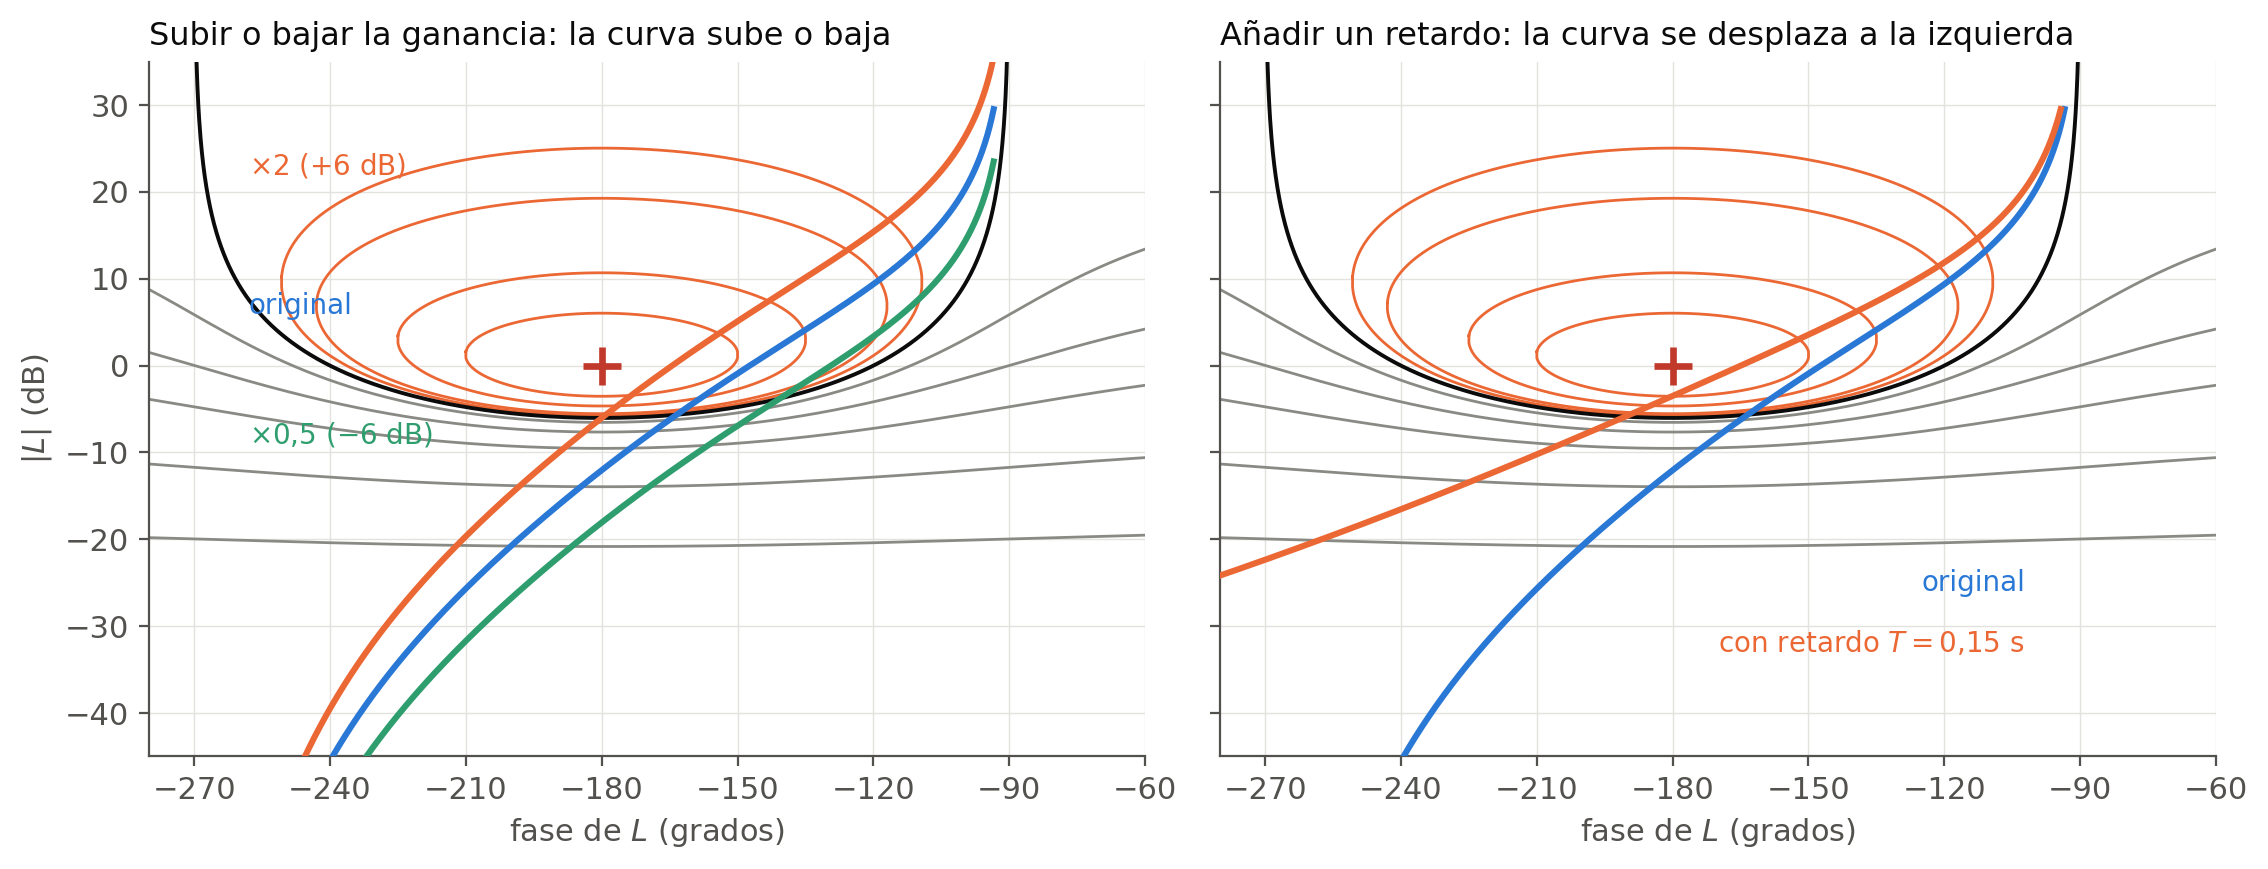
\includegraphics[width=0.88\textwidth]{fig/mover.png}\\[2pt]
  \begin{tabular}{l|c}
    Cambio & Pico de $|T|$\\\hline
    $K$ a la mitad ($-6$ dB) & $1.4$ dB\\
    Original ($K=3$) & $5.1$ dB\\
    $K$ al doble ($+6$ dB) & $11.7$ dB\\
    Retardo $T=0.15$ s & $12.7$ dB
  \end{tabular}
\end{frame}

\begin{frame}{El puente hacia QFT: la incertidumbre es una nube de puntos}
  \footnotesize
  \begin{columns}[T]
  \begin{column}{0.6\textwidth}
    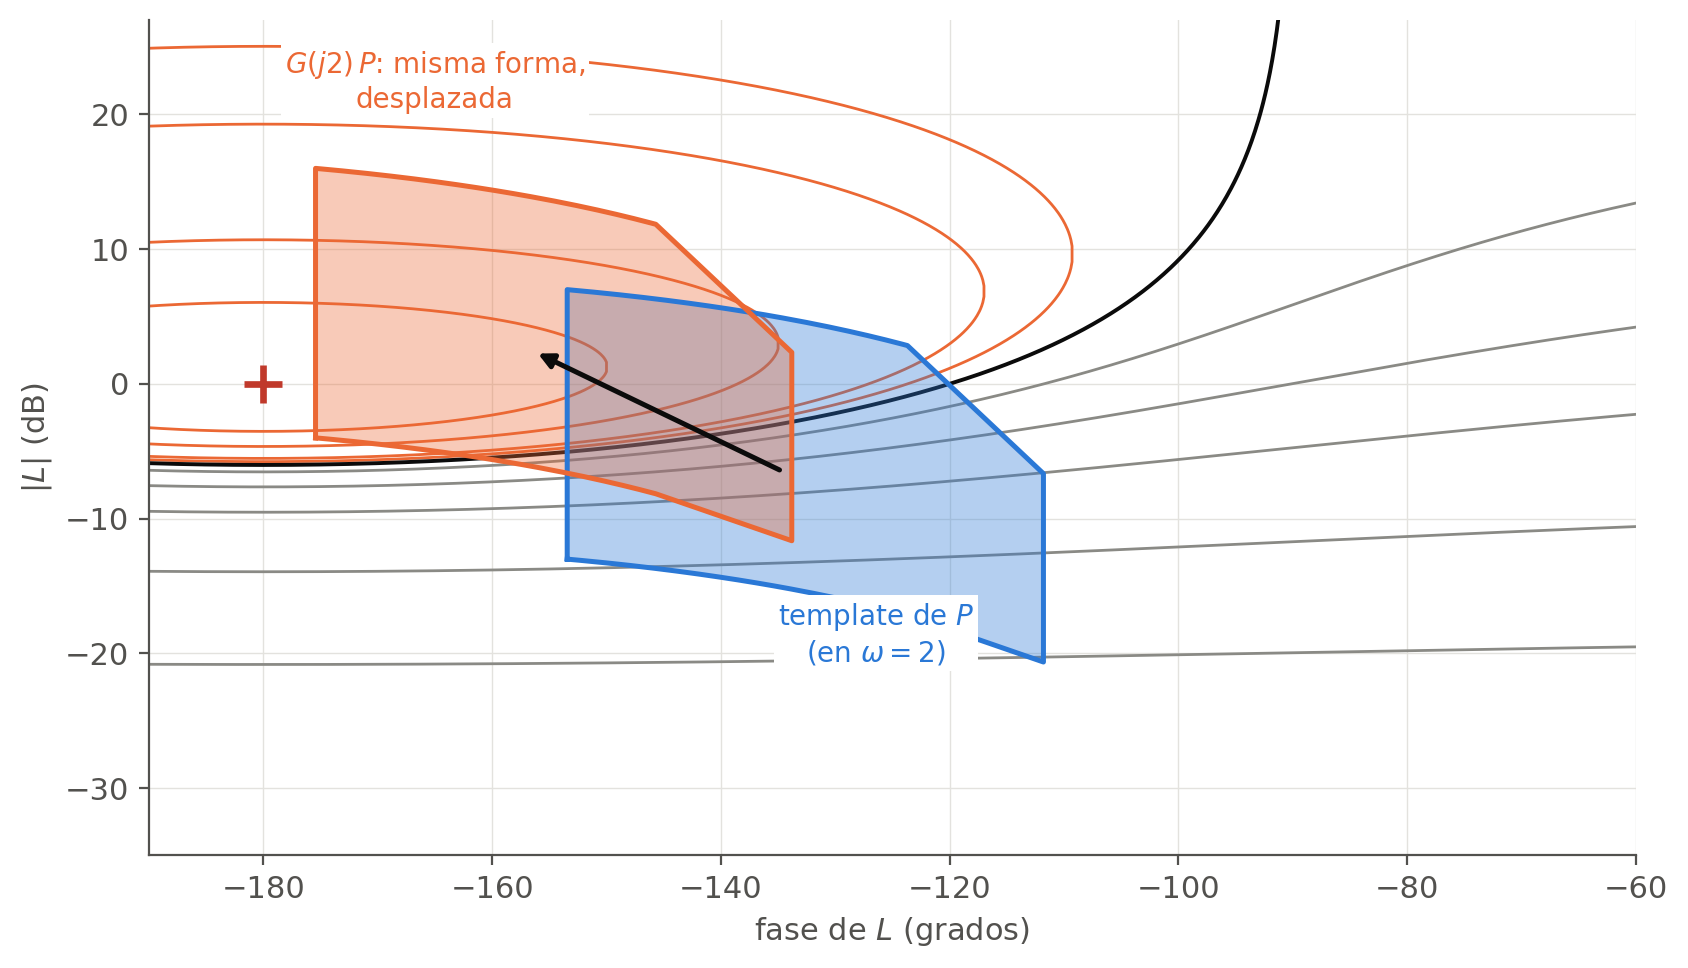
\includegraphics[width=\textwidth]{fig/template.png}
  \end{column}
  \begin{column}{0.38\textwidth}
    Si $P$ no se conoce con exactitud ($P=\frac{K}{s(s+a)}$ con $K\in[1,5]$, $a\in[1,3]$), en cada $\omega$ no hay un punto sino una \textbf{región} en el mapa: el \textbf{template}.
    \begin{block}{Lo que hace $G$}
      Multiplicar por $G(j\omega)$ \textbf{traslada} todo el template sin deformarlo: sumar un vector (fase, dB).
    \end{block}
    \begin{alertblock}{Lo que viene}
      Pasos 7 y 8: construir los templates y, con las especificaciones sobre $|T|$ y $|S|$, trazar los \emph{bounds}: zonas donde el template no puede entrar.
    \end{alertblock}
  \end{column}
  \end{columns}
\end{frame}

\begin{frame}{Ejercicio}
  \small
  En cierta frecuencia $L=1\angle-135^\circ$ (el ejercicio del paso 5).
  \begin{enumerate}
    \item ¿Cuáles son sus coordenadas en el mapa de Nichols?
    \item Sitúalo en la carta y estima $|T|$ por los contornos. Compáralo con el valor calculado en el paso 5: $2.32$ dB.
    \item Súbele $6$ dB al punto ($L=2\angle-135^\circ$) y vuelve a leer. Después bájale $6$ dB. ¿Qué observas?
  \end{enumerate}
  \begin{block}{Pista}
    Las tres posiciones están en la misma vertical, $-135^\circ$.
  \end{block}
  \textcolor{gray}{Solución en el apéndice.}
\end{frame}

\begin{frame}{Para programarlo: el notebook de este paso}
  \small
  Todo lo de este paso se puede \textbf{ejecutar} en el notebook \texttt{notebooks/paso06\_nichols.ipynb}.
  \begin{itemize}
    \item Python: el cambio de coordenadas, la carta de contornos de $|T|$ dibujada desde la ecuación de 2.º grado, los márgenes y los efectos de ganancia y retardo.
    \item Cada cálculo de las diapositivas se \textbf{comprueba} en código, con las mismas cifras.
    \item Incluye celdas \emph{Tu turno} con el ejercicio del paso y la solución plegada.
  \end{itemize}
  \footnotesize Requisitos: \texttt{numpy}, \texttt{scipy}, \texttt{matplotlib}; se abre con \texttt{jupyter lab notebooks/}. Ver \texttt{GUIA.md}.
\end{frame}

\begin{frame}{Resumen}
  \small
  \begin{itemize}
    \item Nichols: $L(j\omega)$ en ejes (fase, dB). El punto $-1$ pasa a ser $(-180^\circ,\ 0\text{ dB})$.
    \item Multiplicar es sumar: ganancia $\Rightarrow$ desplazamiento vertical; retardo $\Rightarrow$ desplazamiento horizontal a la izquierda.
    \item Los contornos de $|T|$ constante vienen de $|T|=\frac{r}{\sqrt{1+2r\cos\theta+r^2}}$ y ya están dibujados en la carta.
    \item Pico de $|T|$ = contorno más alto que toca la curva. Márgenes = distancia al punto crítico.
    \item Siguiente: plantas con incertidumbre. El template será una región de este mapa.
  \end{itemize}
\end{frame}

\appendix
\begin{frame}\centering\Large Apéndice\end{frame}

\begin{frame}{Cómo se dibuja un contorno de $|T|$ constante}
  \footnotesize
  \begin{columns}[T]
  \begin{column}{0.54\textwidth}
    \begin{block}{Procedimiento (un contorno, por ejemplo $6$ dB)}
      \begin{enumerate}
        \item Pasa a lineal: $M=10^{6/20}\approx2$.
        \item Fija una fase $\theta$ y despeja $r=|L|$ de $|T|=M$:
        \[ (1-M^2)\,r^2-2M^2\cos\theta\; r-M^2=0 \]
        \item Quédate con las raíces $r>0$ y pásalas a dB: $20\log_{10}r$.
        \item Repite para muchas fases y une los puntos $(\theta,\,r_{\text{dB}})$.
      \end{enumerate}
    \end{block}
    \textbf{Por qué cierra un óvalo:} para $M>1$ hay solución solo si $\cos^2\theta\ge\frac{M^2-1}{M^2}$ (para $M=2$: $\theta$ entre $-210^\circ$ y $-150^\circ$), y entonces salen dos raíces: la rama de arriba y la de abajo.
  \end{column}
  \begin{column}{0.44\textwidth}
    \centering
    \textbf{Ejemplo $M=2$ (6 dB)}\\[2pt]
    \begin{tabular}{c|cc|cc}
      $\theta$ & $r_{\uparrow}$ & dB & $r_{\downarrow}$ & dB\\\hline
      $-180^\circ$ & $2.00$ & $6.02$ & $0.667$ & $-3.52$\\
      $-170^\circ$ & $1.94$ & $5.75$ & $0.688$ & $-3.25$\\
      $-160^\circ$ & $1.74$ & $4.81$ & $0.767$ & $-2.31$\\
      $-150^\circ$ & $1.15$ & $1.25$ & $1.15$ & $1.25$
    \end{tabular}\\[4pt]
    En $-150^\circ$ las dos ramas se juntan: es el extremo del óvalo.\\[3pt]
    Para $M<1$ (contornos grises) hay una sola raíz positiva a cualquier fase.
  \end{column}
  \end{columns}
\end{frame}

\begin{frame}{Para curiosos: de dónde salen los contornos}
  \small
  Sea $L=x+jy$ y $|T|=M$, es decir $|L|^2=M^2|1+L|^2$:
  \[ x^2+y^2=M^2\big((1+x)^2+y^2\big)\ \Longrightarrow\ \Big(x-\frac{M^2}{1-M^2}\Big)^2+y^2=\frac{M^2}{(1-M^2)^2} \]
  \begin{block}{Es una circunferencia}
    Centro $-\dfrac{M^2}{M^2-1}$ (en el eje real), radio $\dfrac{M}{|M^2-1|}$. Para $M=2$ ($6$ dB): centro $-4/3$, radio $2/3$, así que cruza el eje real en $-2$ y en $-2/3$.
  \end{block}
  Esos dos puntos, en polar: $2\angle-180^\circ$ ($+6.02$ dB) y $0.667\angle-180^\circ$ ($-3.52$ dB), los extremos del óvalo de $6$ dB sobre la vertical de $-180^\circ$ (primera fila de la tabla anterior).\\[3pt]
  \textbf{Resumen:} cada circunferencia del plano complejo, pasada punto a punto a (fase, dB), da un contorno del Nichols.
\end{frame}

\begin{frame}{La misma curva en los dos mapas}
  \footnotesize
  \centering
  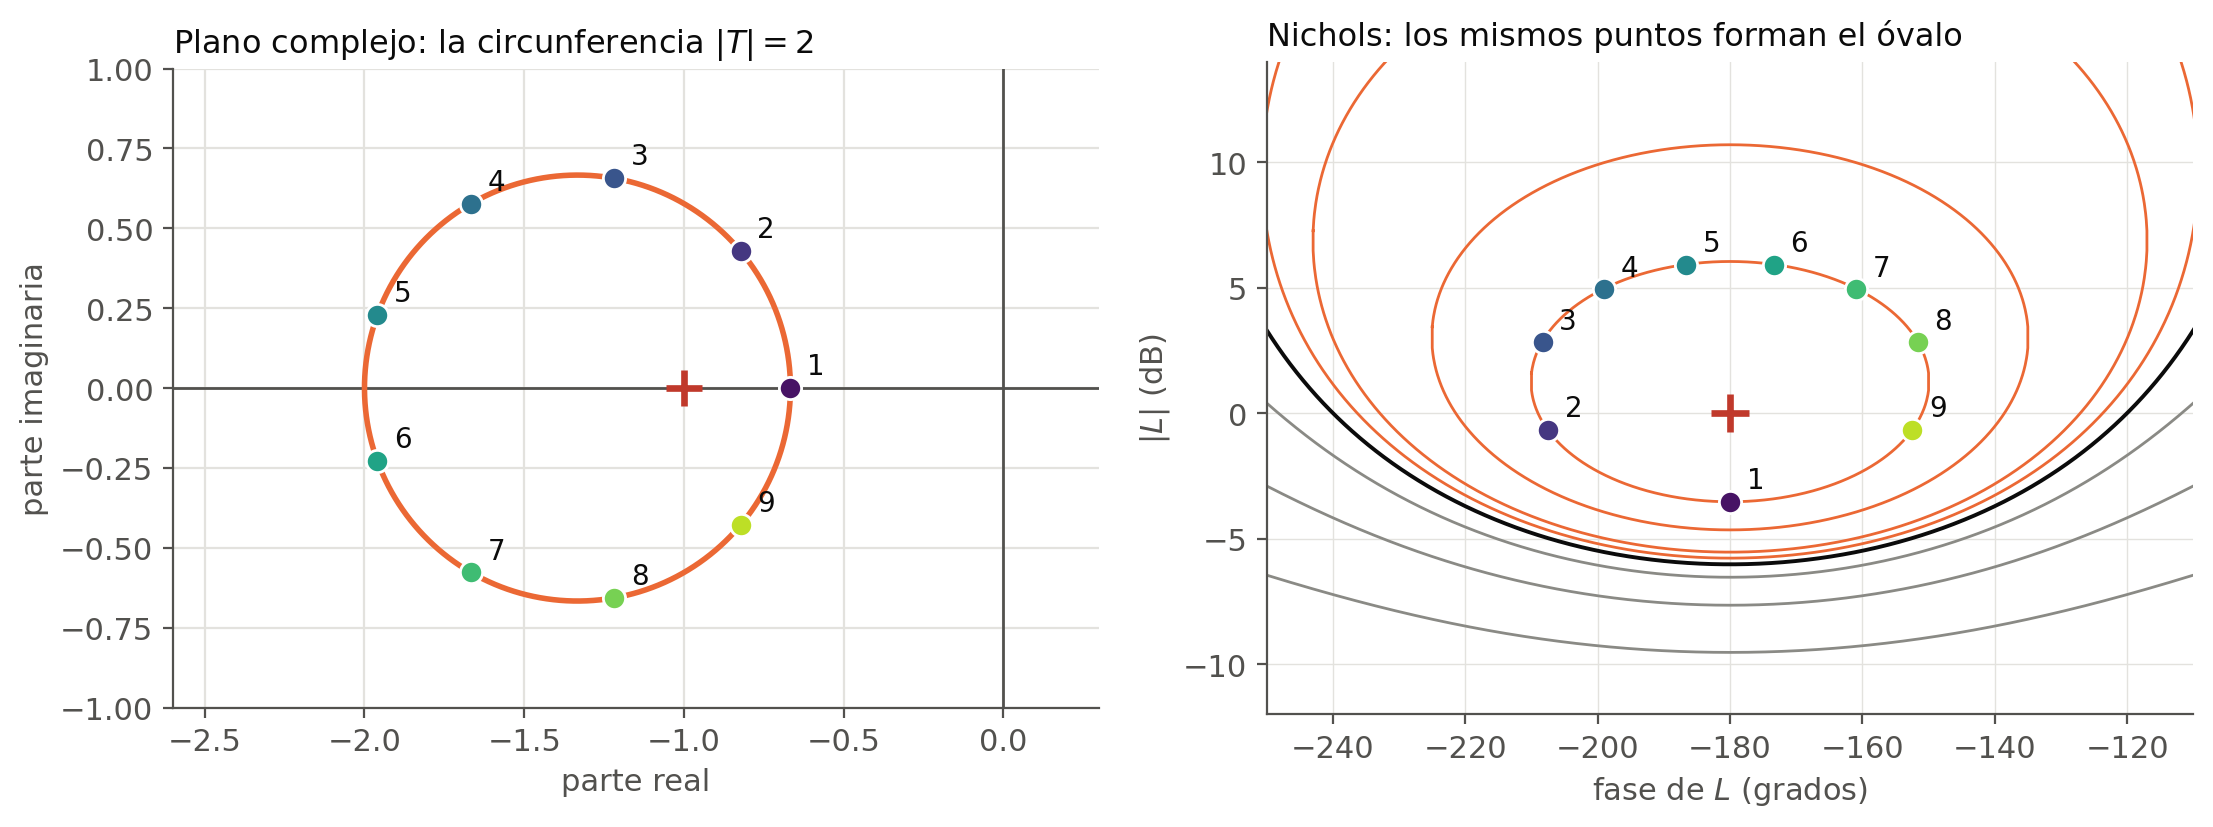
\includegraphics[width=0.95\textwidth]{fig/circulo_ovalo.png}\\[2pt]
  Nueve puntos de la circunferencia $|T|=2$ (izquierda), cada uno convertido a $(\angle L,\ 20\log_{10}|L|)$ (derecha). El punto 1 es el extremo $0.667$ de la tabla; el otro extremo, $2$, cae entre el 5 y el 6.
\end{frame}

\begin{frame}{La otra familia: contornos de fase de $T$ ($\angle T$ constante)}
  \footnotesize
  \begin{columns}[T]
  \begin{column}{0.52\textwidth}
    Con $L=r\angle\theta$ y $T=\frac{L}{1+L}$, conviene invertir:
    \[ \frac1T=1+\frac1L=\frac{(r+\cos\theta)-j\sin\theta}{r} \]
    Si $\angle T=\alpha$, entonces $\angle\frac1T=-\alpha$, y por tanto
    \[ \tan\alpha=\frac{\sin\theta}{r+\cos\theta}\ \Longrightarrow\ \boxed{\,r=\frac{\sin\theta}{\tan\alpha}-\cos\theta\,} \]
    Aquí $r$ sale \textbf{explícito} para cada $\theta$ (no hay cuadrática). Se descartan las soluciones con $r<0$ o con el cuadrante equivocado ($\alpha$ y $\alpha+180^\circ$ comparten tangente).
    \begin{block}{En el plano complejo}
      $\angle T=\alpha$ es otra circunferencia, que pasa por $0$ y por $-1$.
    \end{block}
  \end{column}
  \begin{column}{0.46\textwidth}
    \textbf{Comprobación:} $L=2\angle-200^\circ$ da $\tan\alpha=\dfrac{\sin(-200^\circ)}{2+\cos(-200^\circ)}=\dfrac{0.342}{1.060}$, $\alpha\approx17.9^\circ$. Directo: $1+L=-0.879+0.684j\ (\angle142^\circ)$, $\angle T=-200^\circ-142^\circ=-342^\circ\equiv18^\circ$. Coincide.
    \begin{alertblock}{Para qué se usan}
      En QFT las especificaciones suelen ir sobre $|T|$ y $|S|$, no sobre $\angle T$. Por eso el mapa de los pasos anteriores solo lleva los contornos de $|T|$. La carta clásica imprime ambas familias.
    \end{alertblock}
  \end{column}
  \end{columns}
\end{frame}

\begin{frame}{Los contornos de $\angle T$ sobre la carta}
  \footnotesize
  \begin{columns}[T]
  \begin{column}{0.66\textwidth}
    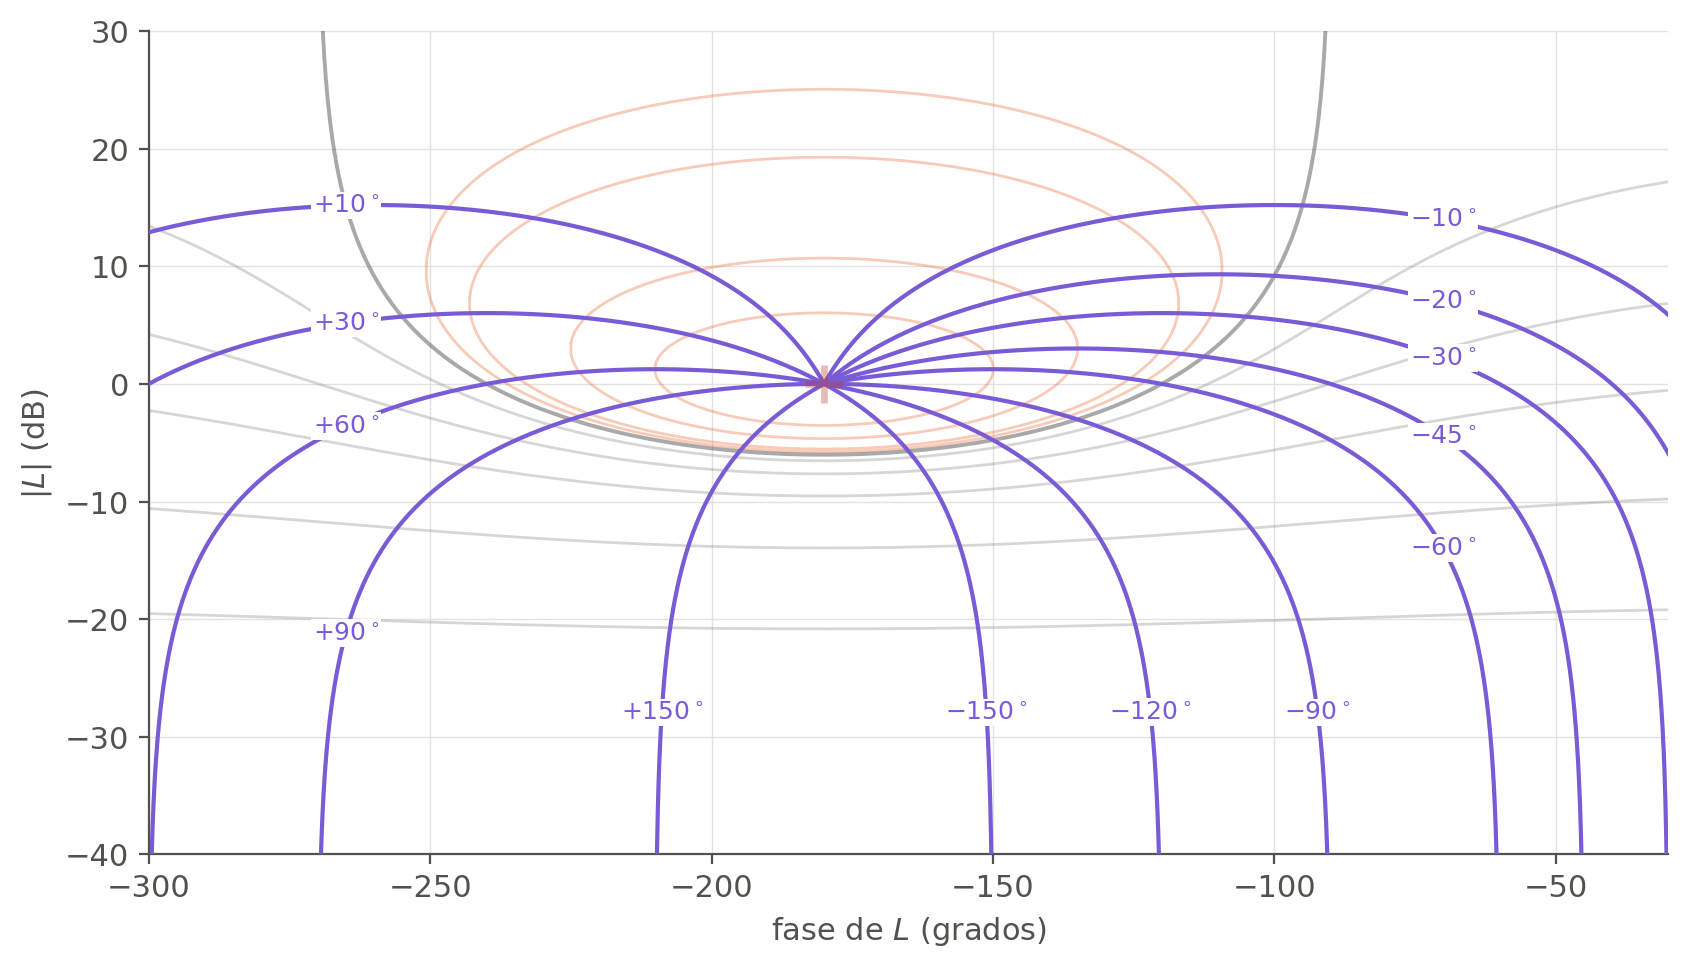
\includegraphics[width=\textwidth]{fig/fase_T.png}
  \end{column}
  \begin{column}{0.32\textwidth}
    \begin{itemize}
      \item Violeta: $\angle T=\alpha$ (valores en grados). Al fondo, los de $|T|$ atenuados.
      \item Todos \textbf{salen del punto crítico}: ahí $1+L=0$ y $\angle T$ no está definido.
      \item A la derecha de $-180^\circ$, $\angle T<0$; a la izquierda, $\angle T>0$.
      \item Lejos del punto, las curvas se vuelven verticales: con $|L|$ pequeño, $T\approx L$ y $\angle T\approx\angle L$.
    \end{itemize}
  \end{column}
  \end{columns}
\end{frame}

\begin{frame}{Solución del ejercicio: $L=1\angle-135^\circ$}
  \small
  \textbf{1.} $(\angle L,\ |L|_{\text{dB}})=(-135^\circ,\ 0\text{ dB})$.\\[3pt]
  \textbf{2.} Con $r=1$, $\theta=-135^\circ$: $|T|=\dfrac{1}{\sqrt{2+2\cos(-135^\circ)}}=\dfrac{1}{\sqrt{0.586}}=1.307\to2.32$ dB. En la carta cae entre los óvalos de $1$ y $3$ dB.\\[3pt]
  \textbf{3.} Subir $6$ dB ($r=2$): $|T|=2.65$ dB. Bajar $6$ dB ($r=0.5$): $|T|=-3.37$ dB.\\[6pt]
  \begin{block}{Observación}
    Con la fase fija en $-135^\circ$, $|T|$ \textbf{aumenta} al subir la ganancia pero con rendimientos decrecientes ($2.32\to2.65$ dB): $L$ se aleja del origen, pero ya está lejos de $-1$ en esa fase. A la baja, $|T|\approx|L|$ y cae casi dB por dB.
  \end{block}
\end{frame}
\end{document}
